\chapter{Unsch"arfeprinzip der Fourier-Transformation \label{chapter:heisenbergfourier}}
\lhead{Heisenberg Unsch"arfe}
\begin{refsection}
\chapterauthor{Dorian Amiet}
\rhead{Fourier Transformation}

Das im Kapitel \ref{chapter:heisenberg} hergeleitete Unsch"arfeprinzip von Heisenberg beruht, rein mathematisch betrachtet, auf einer grundlegenden Eigenschaft der Fourier-Transformation.
Bemerkenswert ist, dass die Theorie zur Fourier-Transformation bereits "uber hundert Jahre alt war, als Heisenberg die Unsch"arfe entdeckte.
In diesem Kapitel werden die f"ur das Unsch"arfeprinzip wesentlichen Punkte der Fourier Transformation erl"autert sowie die physikalischen Folgen aufgezeigt.

\section{Die Fourier Transformation}

Die kontinuierliche Fourier-Transformation ist eine Methode der Fourier-Analysis, die es erlaubt, kontinuierliche, aperiodische Signale in ein kontinuierliches Spektrum zu zerlegen.
Die Funktion, die dieses Spektrum beschreibt, nennt man auch Fourier Transformierte oder Spektralfunktion.
Diese Integraltransformation ist benannt nach dem Mathematiker Jean Baptiste Joseph Fourier, der im Jahr 1822 die Fourier-Reihen einf"uhrte, ein Analogon der kontinuierlichen Fourier Transformation f"ur periodische Signale.

\subsection{Definition}

Die Fourier-Transformation einer Funktion $\hat{f}=\mathcal{F}(f)$ ist definiert, wenn das Integral
\begin{equation}
\hat{f}(k) := \dfrac{1}{\sqrt{2\pi}}\int_{-\infty}^{\infty}e^{-i k x} \, f(x) \; dx \qquad \textnormal{f"ur } k \in \mathbb{R}
\end{equation}
existiert.
Anstelle von $\hat{f}=\mathcal{F}(f)$ findet sich in der Literatur auch die Schreibweise
%$f \circ\,\!\! \!\!-\!\!\!-\!\!\!\bullet \hat{f}$.
$f \multimapdotbothA \hat{f}$.
Die inverse Fourier-Transformation $f=\mathcal{F}^{-1}(\hat{f})$ ist symmetrisch. Nur die Variablen $k$ und $x$ sind vertauscht.
\begin{equation}
f(x) := \dfrac{1}{\sqrt{2\pi}}\int_{-\infty}^{\infty}e^{-i k x} \, \hat{f}(k) \; dk \qquad \textnormal{f"ur } x \in \mathbb{R}
\end{equation}
In der Literatur ist auch der Vorfaktor $\dfrac{1}{\sqrt{2\pi}}$ unterschiedlich. Eine h"aufig anzutreffen Variante ist, wenn der Faktor $\dfrac{1}{\sqrt{2\pi}}$ mit $\dfrac{1}{2\pi}$ ersetzt und nur bei der R"ucktransformation angewendet wird.
Hier wird $\dfrac{1}{\sqrt{2\pi}}$ verwendet, weil es f"ur die sp"atere physikalische Analyse einfacher ist.

\subsection{Beispiel}

An einem simplen Beispiel wird gezeigt, wie die Fourier Transformierte auf eine Funktion wirkt. Dazu betrachten wir die Funktion
\begin{equation}
f(x)=\begin{cases}
    \frac{1}{\sqrt{2\tau}}       & \qquad |x|< \tau \;\;\; \textnormal{f"ur }  \tau > 0\\
    0  & \qquad\text{sonst.}\\
  \end{cases}
\end{equation}
und berechnen davon die Fourier-Transformation. $\hat{f}=\mathcal{F}(f)$
\begin{align}
\hat{f}(k)
&=\dfrac{1}{\sqrt{2\pi}}\int_{-\infty}^{\infty}e^{-i k x} \, f(x) \; dx\\
&=\dfrac{1}{\sqrt{2\pi}}\int_{-\tau}^{\tau}e^{-i k x} \, \frac{1}{\sqrt{2\tau}} \; dx\\
&=\dfrac{1}{\sqrt{2\pi}}\frac{1}{\sqrt{2\tau}}\left[ \dfrac{i}{k}e^{-ik x}\right]_{-\tau}^{\tau}\\
&=\dfrac{1}{2\sqrt{\tau\pi}}\dfrac{i}{k}\left[e^{-ik \tau} - e^{ik \tau}\right]\\
&=\dfrac{1}{2\sqrt{\tau\pi}}\dfrac{2}{k}\dfrac{e^{-ik \tau} - e^{ik \tau}}{2i}\\
&=\dfrac{1}{\sqrt{\tau\pi}}\dfrac{1}{k}\sin(\tau k)\\
&=\sqrt{\frac{1}{\tau\pi}}\dfrac{\sin(\tau k)}{k}
\end{align}
\begin{figure}
 \centering
 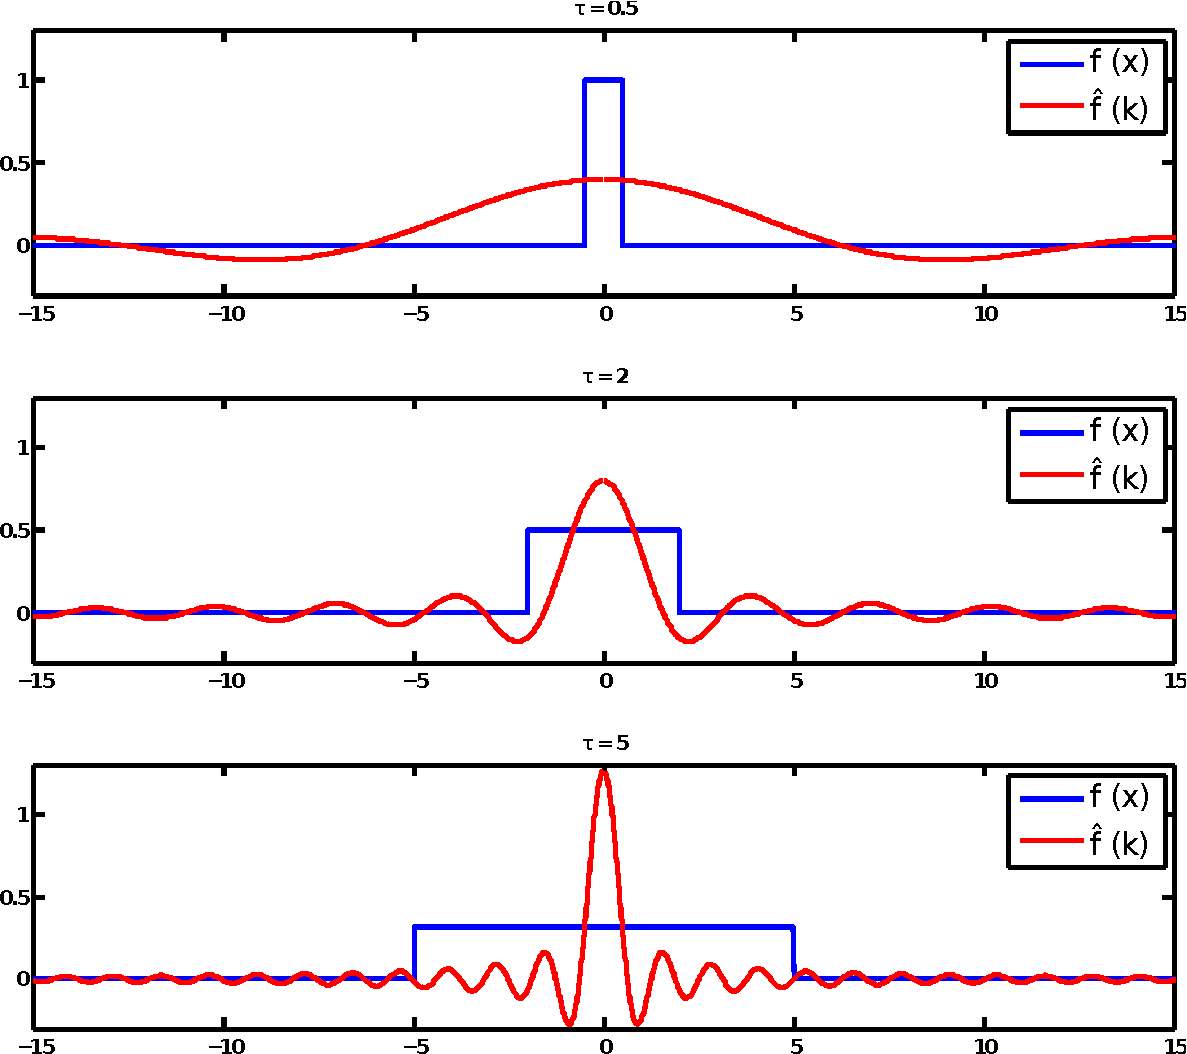
\includegraphics[width=12cm]{heisenberg/fourier_unschaerfeprinzip.pdf}
 \caption{Breites $f(x)$ f"uhrt zu schmalem $\hat{f}(k)$}
 \label{abb:unschaerfeprinzip}
\end{figure}
Werden die beiden Funktionen mit verschiedenen $\tau$ gezeichnet (Abbildung \ref{abb:unschaerfeprinzip}), wird das Unsch\"arfeprinzip erkennbar. Je breiter $f(x)$, desto schmaler wird $\hat{f}(k)$. Analog gilt, dass ein breiteres $\hat{f}(k)$ ein schmaleres $f(x)$ zur Folge hat.

Die Relationen der Breite und Amplituden der Fourier Transformierten gelten allgemein. F"ur ein beliebiges reelles $a$ gilt
\begin{equation}
\mathcal{F}(f(ax)) = \frac{1}{|a|}\cdot\hat{f}\left( \frac{k}{a}\right) 
\end{equation}
Aufgrund der Symmetrie gilt auch das umkehrte
\begin{equation}
\hat{f}(ak) = \mathcal{F}\left( \frac{1}{|a|}f\left( \frac{x}{a}\right) \right) 
\end{equation}
Eine weitere Eigenschaft ist die Normerhaltung. Das heisst
\begin{equation}
\int_{-\infty}^{\infty}|f(x)|^{2} \, dx = \int_{-\infty}^{\infty}|\hat{f}(k)|^{2} \, dk
\end{equation}
Unser Beispiel ist so gew"ahlt, dass
\begin{equation}
\int_{-\infty}^{\infty}|f(x)|^{2} \, dx = 1 = \int_{-\infty}^{\infty}|\hat{f}(k)|^{2} \, dk
\end{equation}
Ursache f"ur diese Normerhaltung ist die Tatsache, dass es sich bei der Fourier Transformation um eine unit"are Abbildung handelt.
Ein Beweis daf"ur kann in \cite{skript:QuantenmechanikMotschmann} nachgeschlagen werden.

\subsection{Differentiation}
\label{chapter:ftrans_differentation}

Weiter untersuchen wir, welche Operation im Spektrum der Ableitung im Zeitbereich entspricht.
Sei $f(x)$ eine (differenzierbare) Zeitfunktion mit der Fourier transformierten $\hat{f}(k)$
\begin{equation}
\mathcal{F}(f(x)) = \hat{f}(k)
\end{equation}
Die Ableitung $f'(x)$ k"onnen wir in die Definition einsetzen und das resultierende Integral partiell integrieren. 
\begin{align}
\mathcal{F}(f'(x)) &= \dfrac{1}{\sqrt{2\pi}}\int_{-\infty}^{\infty}e^{-i k x} \, f'(x) \; dx\\
&= \dfrac{1}{\sqrt{2\pi}}\left[f(x)\cdot e^{-i k x} \right]_{-\infty}^{\infty}-  \dfrac{1}{\sqrt{2\pi}}(-ik)\cdot\int_{-\infty}^{\infty}e^{-i k x} \, f(x) \; dx
\end{align}
Wenn die Funktion $f(x)$ f"ur $x \rightarrow \pm \infty$ gegen Null geht, bleibt nur noch die Fourier transformierte und ein Faktor "ubrig.
$f(x) = 0$ f"ur  $x \rightarrow \pm \infty$ ist keine Einschr"ankung von $f(x)$.
Andernfalls w"are die Fourier Transformation sowieso nicht anwendbar.
Es bleibt "ubrig
\begin{equation}
\mathcal{F}(f'(x))= \dfrac{ik}{\sqrt{2\pi}}\int_{-\infty}^{\infty}e^{-i k x} \, f(x) \; dx
\end{equation}
respektive
\begin{equation}
\mathcal{F}(f'(x))= ik\cdot\hat{f}(k)
\end{equation}
Eine Differentiation entspricht einer Multiplikation in der Fourier Transformierten.
Aufgrund der Symmetrie gilt dies nat"urlich auch in Gegenrichtung.
\begin{equation}
ix\cdot(f(x))= \mathcal{F}(\hat{f'}(k))
\end{equation}

\section{$k$-Darstellung}
\rhead{$k$-Darstellung}


Wir kennen die Ortsdarstellung aus dem Kapitel \ref{chapter:quantisierung}.
Um die weiteren Rechnungen zu vereinfachen, wird die Wellenzahl $k$ definiert.
\begin{equation}
k := \frac{p}{\hbar}
\end{equation}
Wir versuchen nun, von der Ortsdarstellung in die $k$-Darstellung "uber zu gehen.
Dies bedeutet, dass ein Basiswechsel von $\vert x\rangle$ zu $\vert k\rangle$ gemacht wird.
Mit Hilfe von
\begin{equation}
\langle x\vert k\rangle= \langle k\vert x\rangle =\frac{1}{\sqrt{2\pi }}e^{-ikx} 
\end{equation}
gelangen wir von der einen in die andere Darstellung.
Ein bestimmter Ket $|\psi\rangle$ wird in Ortsdarstellung durch $\langle x\vert \psi\rangle = \psi(x)$ und in der $k$-Darstellung durch $\langle k\vert \psi\rangle = \hat{\psi}(k)$ repr"asentiert.
\begin{align}
\langle x\vert \psi\rangle &= \int_{-\infty}^{\infty} \langle x\vert k\rangle \langle k\vert \psi\rangle \; dk\\
&=\int_{-\infty}^{\infty} \frac{1}{\sqrt{2\pi }}e^{-ikx}  \langle k\vert \psi\rangle \; dk\\
&= \frac{1}{\sqrt{2\pi }} \int_{-\infty}^{\infty} e^{-ikx}  \langle k\vert \psi\rangle \; dk\\
\psi(x) &= \frac{1}{\sqrt{2\pi }} \int_{-\infty}^{\infty} e^{-ikx} \hat{\psi}(k) \; dk
\end{align}
Das Resultierende entspricht genau der Fourier Transformation.
Umkehrt ist
\begin{align}
\langle k\vert \psi\rangle &= \int_{-\infty}^{\infty} \langle k\vert x\rangle \langle x\vert \psi\rangle \; dx\\
\hat{\psi}(k) &= \frac{1}{\sqrt{2\pi}} \int_{-\infty}^{\infty} e^{-ikx} {\psi}(x) \; dx
\end{align}
In der Ortsdarstellung kennen wir bereits den Ortsoperator
\begin{equation}
 x \cdot\psi(x)
\end{equation}
Weiter wird in Satz \ref{skript:quantisierungsregeln-ortsdarstellung} der Impulsoperator in Ortsdarstellung beschrieben. Er ist
\begin{equation}
 \hat p  =\frac{\hbar}{i}\frac{\partial}{\partial x}
\end{equation}
Setzten wir das $k$ in den Impulsoperator ein, verschwindet das $\hbar$
\begin{equation}
\hat p_{k} = -i\frac{\partial}{\partial x}
\end{equation}
Ausserdem rechnen wir die Operatoren f"ur Impuls und Ort in die $k$-Darstellung um.
Dabei ber"ucksichtigen wir, dass die Fourier Transformation eine Multiplikation mit x durch eine Ableitung nach k umwandelt.
\begin{align}
x\cdot\psi(x) &= \frac{1}{\sqrt{2\pi }} \int_{-\infty}^{\infty} e^{-ikx} x \;\hat{\psi}(k) \; dk\\
&= \frac{1}{\sqrt{2\pi }} \int_{-\infty}^{\infty} e^{-ikx} \frac{1}{i}\frac{\partial}{\partial k} \hat{\psi}(k) \; dk
\end{align}
Der Ortsoperator in k-Darstellung ist 
\begin{equation}
\frac{1}{i}\frac{\partial}{\partial k}
\end{equation}
In der folgenden Tabelle sind die verschiedenen Operatoren in Orts- und $k$-Darstellung zusammengefasst.
\begin{center}
\renewcommand{\arraystretch}{1.25}
\begin{tabular}{|l|c|c|}
\hline
& Ortsdarstellung & $k$-Darstellung\\
\hline
Ortsoperator & $x \cdot \psi(x) $ & $\frac{1}{i}\frac{\partial}{\partial k} \cdot \hat{\psi}(k)$\\
 \hline
Impulsoperator & $\frac{\hbar}{i}\frac{\partial}{\partial x} \cdot \psi(x)$ & $\hbar \cdot k \cdot \hat{\psi}(k)$\\
\hline
\end{tabular}
\renewcommand{\arraystretch}{1}
\end{center}

\subsection{Unsch"arferelation}

Da der Impuls und Ortsoperator "uber die Fouriertransformation zusammen verkn"upft sind, sollte die Unsch"arferelation berechnet werden k"onnen, indem zwei Wahrscheinlichkeitsdichterfunktionen "uber die Fouriertransformation miteinander verkn"upft werden.
Wir nehmen eine Quadratisch integrierbare Funktion und normieren diese auf 1.
\begin{equation}
	\int_{-\infty}^{\infty} |f(x)|^{2} \; dx = 1
\end{equation}
Wir interpretieren $|f(x)|^{2}$ als eine Wahrscheinlichkeitsdichtefunktion mit Mittelwert 0 und Varianz $V(f)$.
\begin{equation}	
	\text{var}(f) = \varDelta X^{2} = \int_{-\infty}^{\infty} (x)^{2} \cdot |f(x)|^{2} \; dx
	\label{equation:varianz1.0}
\end{equation}
Es gilt die Cauchy-Schwarz-Ungleichung
\begin{equation}	
	\left| \int_{-\infty}^{\infty} x \overline{f(x)}  f'(x) \; dx\right|^{2} \leq  \int_{-\infty}^{\infty} \left| x f(x)\right|^{2}\; dx \cdot \int_{-\infty}^{\infty} \left| f'(x)\right|^{2}\; dx
	\label{equation:Cauchy_Schwarz}
\end{equation}
F"ur die Linke Seite m"ussen wir eine Absch"atzung nach unten machen.
Diese kann partiell integriert werden.
\begin{equation}	
	\int_{-\infty}^{\infty} x \overline{f(x)}  f'(x) \; dx = \left[ x \overline{f(x)}f(x) \right]_{-\infty}^{\infty}-  \int_{-\infty}^{\infty} \overline{f(x)}f(x) +  x \overline{f'(x)}  f(x)\; dx
\end{equation} 
Der erste Teil gibt Null und vom zweiten Teil gen"ugt der Realteil.
\begin{align}	
\left| \int_{-\infty}^{\infty} x \overline{f(x)}  f'(x) \; dx\right|^{2}
&= \left| -  \int_{-\infty}^{\infty} \overline{f(x)}f(x) +  x \overline{f'(x)}  f(x)\; dx\right| ^{2}\\
&\geq \left| \text{Re}\left\lbrace -\int_{-\infty}^{\infty} \overline{f(x)}f(x)\; +  x \overline{f'(x)}  f(x)\; dx \right\rbrace\right|^{2}\\
&\geq\left| -\dfrac{1}{2} \int_{-\infty}^{\infty} \left| f(x)\right|^{2}\; dx \right|^{2}\\
&\geq \frac{1}{4}
\end{align}
Nun haben wir von der linken Seite der Formel \ref{equation:Cauchy_Schwarz} eine Absch"atzung gegen unten.
Die rechte Seite ist die Multiplikation zwischen der Varianz von $f(x)$ und einem zweiten Teil, den wir noch genauer analysieren.
Wir berechnen die Fourier Transformierte von $f'(x)$.
\begin{equation}	
\mathcal{F}(f'(x)) = ik \cdot \hat{f}(k)
\end{equation}
Aufgrund der Normerhaltung gilt
\begin{equation}	
\int_{-\infty}^{\infty} \left| f'(x)\right|^{2}\; dx = \int_{-\infty}^{\infty} \left| ik \hat{f}(k)\right|^{2}\; dk= \int_{-\infty}^{\infty} \left| k \hat{f}(k)\right|^{2}\; dk
\end{equation}
Dies entspricht gerade der Varianz der Fourier Transformierten von $f(x)$. Wir setzen die Erkenntnisse in \ref{equation:Cauchy_Schwarz} ein und erhalten

\begin{equation}
\frac{1}{4}\leq \int_{-\infty}^{\infty} \left| x f(x)\right|^{2}\; dx \cdot \int_{-\infty}^{\infty} \left| k \hat{f}(k)\right|^{2}\; dk
\end{equation}
oder

\begin{equation}
\varDelta X^{2}\cdot\varDelta K^{2}\geq\frac{1}{4}
\end{equation}
Wird das $k$ durch seine Definition $k = \frac{p}{\hbar}$ ersetzt, erhalten wir die Unsch"arferelation, wie wir sie bereits aus Kapitel \ref{chapter:heisenberg} kennen.
\begin{equation}
\varDelta X^{2}\cdot\varDelta P^{2}\geq\frac{\hbar^{2}}{4}
\label{equation:ort_impuls_unschaerfe}
\end{equation}

\subsection{Gaussverteilung}

Wir machen ein Beispiel zur Unsch"arfe der Fourier Transformation und nehmen als Wahrscheinlichkeitsdichtefunktion eine Gaussverteilung an.
Diese ist quadratisch integrierbar und deren Norm ist 1.
\begin{equation}
	\int_{-\infty}^{\infty} |f(x)|^{2} \; dx = 1
\end{equation}
Die Wahrscheinlichkeitsdichtefunktion ist $|f(x)|^{2}$ und hat Mittelwert $\mu$ und Varianz $V(f)$.
\begin{equation}
	\mu = \int_{-\infty}^{\infty} x \cdot |f(x)|^{2} \; dx
\end{equation}
\begin{equation}	
	\text{var}(f) = \varDelta X^{2} = \int_{-\infty}^{\infty} (x-\mu)^{2} \cdot |f(x)|^{2} \; dx
	\label{equation:varianz1}
\end{equation}
Wir setzen f"ur $|f(x)|^{2}$ eine gausssche Dichtefunktion mit $\mu = 0$ ein.
\begin{equation}
	|f(x)|^{2}  = \dfrac{1}{\sigma \sqrt{\pi}}e^{-\frac{x^{2}}{\sigma^{2}}}
\end{equation}
Durch Wurzel ziehen kann $f(x)$ bestimmt werden
 \begin{equation}
 	f(x) =\dfrac{1}{\sqrt{\sigma\sqrt{\pi}} }e^{-\frac{x^{2}}{2\sigma}} 
 \end{equation}
Davon wird die Fourier transformierte berechnet
 \begin{equation}
 	\mathcal{F}(f(x)) = \hat{f}(k) = \sqrt{\dfrac{\sigma}{\sqrt{\pi}} }e^{-\frac{\sigma^{2} k^{2}}{2}}
 \end{equation}
Die Wahrscheinlichkeitsdichtefunktion $|\hat{f}(k)|^{2}$ ergibt sich aus dem Absolutquadrat von $\hat{f}(k)$.
\begin{equation}
	|\hat{f}(k)|^{2} = \dfrac{\sigma}{\sqrt{\pi} }e^{-\sigma^{2} k^{2}}
	\label{equation:fourier_gauss}
\end{equation}
Dass $|\hat{f}(k)|^{2}$ eine Wahrscheinlichkeitsdichtefunktion ist, kann durch Integration "uberpr"uft werden.
\begin{equation}
	\int_{-\infty}^{\infty}  |\hat{f}(k)|^{2} \; dk = \int_{-\infty}^{\infty} \dfrac{\sigma}{\sqrt{\pi} }e^{-\sigma^{2} k^{2}} \; dk = 1
\end{equation}
Bei genauerer Betrachtung von Formel \ref{equation:fourier_gauss} ist ersichtlich, dass es sich bei $|\hat{f}(k)|^{2}$ wieder um eine Gaussverteilung handelt, wobei $\sigma$ durch $\frac{1}{\sigma}$ ersetzt wurde.
Analog zu $f(x)$ kann auch von $\hat{f}(k)$ den Mittelwert und die Varianz berechnet werden.
\begin{equation}
	\hat{\mu} = \int_{-\infty}^{\infty} k \cdot  |\hat{f}(k)|^{2}\; dk
\end{equation}
\begin{equation}	
	\text{var}(\hat{f}) = \varDelta K^{2}  = \int_{-\infty}^{\infty} (k-\mu)^{2} \cdot  |\hat{f}(k)|^{2} \; dk
	\label{equation:varianz2}
\end{equation}
Mit den Formeln \ref{equation:varianz1} und \ref{equation:varianz2} k"onnen nun die Varianzen der beiden Funktionen $f(x)$ und $\hat{f}(k)$ berechnet werden.
\begin{equation}	
	\varDelta X^{2} = \int_{-\infty}^{\infty} x^{2} \cdot \dfrac{1}{\sigma \sqrt{\pi}}e^{-\frac{x^{2}}{\sigma^{2}}} \; dx = \frac{\sigma^{2}}{2}
\end{equation}
\begin{equation}	
	\varDelta K^{2} = \int_{-\infty}^{\infty} (k-\mu)^{2} \cdot  \dfrac{\sigma}{\sqrt{\pi} }e^{-\sigma^{2} k^{2}} \; dk = \dfrac{1}{2\sigma^{2}}
\end{equation}
Die beiden Varianzen werden multipliziert
\begin{equation}	
	\varDelta X^{2} \cdot \varDelta K^{2} = \frac{\sigma^{2}}{2} \cdot \dfrac{1}{2\sigma^{2}} = \dfrac{1}{4}
\end{equation}
Wird das $k$ durch $\frac{p}{\hbar}$ ersetzt, so kommt die Unsch"arfere f"ur Impuls und Ort heraus.
\begin{equation}	
	\varDelta X^{2} \cdot \varDelta P^{2} = \dfrac{\hbar^{2}}{4}
\end{equation}
Wir konnten zeigen, dass die Ungleichung \ref{equation:ort_impuls_unschaerfe} mit Gleichheit erf"ullt wird, wenn als Wahrscheinlichkeitsdichtefunktion eine Gaussverteilung angenommen wird.
Es ist sogar so, dass die Normalverteilung die einzige Verteilung mit dieser Eigenschaft ist.

\subsection{Fazit}

Die Unsch"arferelation ist eine gegebene Sache. Egal wie genau ein Messger"at je gebaut wird, die Unsch"arfe von $\varDelta X \cdot \varDelta P \geq \dfrac{\hbar}{2}$ bleibt. Das genaust m"ogliche Resultat wird erzielt, wenn die Verteilung der Teilchen normalverteilt angenommen werden. Dann wird die Ungleichung mit Gleichheit erf"ullt.

\printbibliography[heading=subbibliography]
\end{refsection}

